\section{이론적 배경}

\subsection{천체 관측 시스템}

Fig. \ref{fig:observing_system}\은 관측 환경이 좋은 곳으로 망원경을 이동하여 사진 관측을 할 수 있는 소형 천체 망원경 시스템을 보여 준다. 사진 관측을 위한 천체 망원경 시스템은 크게 광학계(optic), 검출기(detector), 마운트(mount)로 이루어지며, 정밀도를 높이기 위해 가이드 시스템을 포함한 여러가지 보조 도구들이 필요하다. 광학계의 결상 성능, 마운트의 추적 성능 등을 갖추고 있어야 오랜 시간동안 노출을 주며 천체 사진을 찍을 수 있게 된다. 

앞서 제시한 Fig. \ref{fig:The_Andromeda_Galaxy}의 안드로메다 은하 사진은 Fig. \ref{fig:observing_system}\을 이용하여 촬영한 것이다. 상세 정보를 보면 Sbig(Santa Barbara Instrument Group)사의  ST-8300M이라는 모노크롬 CCD(Charge-coupled device)를 이용하여 촬영하였으며, 노출 정보를 보면 L(Luminence) 채널의 경우 600 sec의 노출로 14 frame을 촬영하여 합성하였으며, R(Red), G(Green), B(Blue) 각각의 채널에서 400 sec의 노출로 6 frame씩 촬영하여 합성한 것이다. 이처럼 고품질의 천체사진 한 장을 촬영하기 위해서 많은 시간과 노력이 필요하다. 

\begin{figure}[h]
	\begin{center}
	\begin{tikzpicture}
		\node[anchor=south west,inner sep=0] at (0,0) {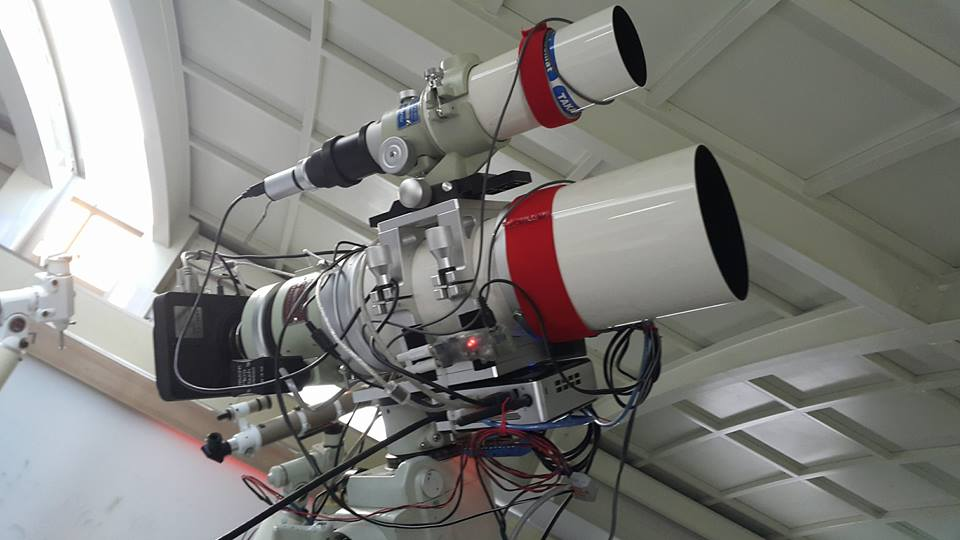
\includegraphics[width=0.8\textwidth]{observing_system}};
		\draw[->, -stealth, draw=red, line width=0.7mm] (11.2, 2.8) --++ (-1.5, 0.7);
		\node[rectangle, draw, fill=black!10, minimum size=0.5] at (11.2, 2.8) {(a)};
		\draw[->, -stealth, draw=red, line width=0.7mm] (0.8, 2.8) --++ (1.2, 0.2);
		\node[rectangle, draw, fill=black!10, minimum size=0.5] at (0.8, 2.8) {(b)};
		\draw[->, -stealth, draw=red, line width=0.7mm] (10.2, 6.1) --++ (-1.5, 0.2);
		\node[rectangle, draw, fill=black!10, minimum size=0.5] at (10.2, 6.1) {(c)};
		\draw[->, -stealth, draw=red, line width=0.7mm] (2.8, 5.5) --++ (1.2, -0.2);
		\node[rectangle, draw, fill=black!10, minimum size=0.5] at (2.8, 5.5) {(d)};
	\end{tikzpicture}
	\end{center}
	\caption{A Small Telescope observing system for astrophotography : (a) main optic, (b) CCD, (c) guide optic, (d) guide CCD}
	\label{fig:observing_system}
\end{figure}


\subsection{사진 관측에서 초점 조절}

사진 관측에서 별의 초점을 조절하는 알고리즘 중 가장 많이 사용하는 것이 HFD(Half Flux Diameter) 값을 이용하는 것이다. FocusMAX 프로그램에서 각각의 프레임을 얻은 후 HFD를 측정하는 알고리즘은 다음과 같다 \cite{weber2001fast}.

1. 이미지에서 배경 레벨을 빼준다. 

2. 간단한 가중치 평균법으로 별의 중심을 구한다.

3. 중심에서 각 픽셀의 반지름을 결정한다. 

4. 반지름이 커지는 순서대로 픽셀을 정렬한다. 

5. 지름을 따라 픽셀 플럭스의 적분을 구한다. 적분은 사용자 양식에서 찾기 및 초점 버튼 왼쪽에 작은 플롯으로 표시됩니다. 가로 축을 따라 지름과 세로 축을 따라 플럭스를 플로팅한다. 적분은 제로 직경에서 제로 통합 플럭스를 나타내고 최대 직경에서 전체 스타 플럭스를 나타낸다. 

6.이 적분에서 절반 플럭스 지름을 결정한다. 이는 단순히 통합 플럭스가 전체 스타 플럭스의 절반인 지름이다. 이 HFD 포인트는 플럭스 적분 플롯에 수직선으로 표시된다. 

그 외에도 FWHM (Full Width Half Maximum) 을 측정하여 이용할 수도 있으나 별의 플럭스가 정규 분포를 따르지 않을 때는 사용하기 어렵다는 단점이 있다. 

FWHM 값이나 HFD 값 모두 최솟값을 나타낼 때가 초점이 가장 잘 맞았을 때이다. 따라서 모터 포커서를 일정한 간격으로 움직이며 HFD 값을 구하여 플로팅을 해보면 V curve를 그리게 된다. FocusMAX에서는 다음과 같이  V curve를 그려 자동으로 초점을 조절하고 있다. \cite{weber2001fast}.

1. 처음에는 초점이 맞지 않은 상태에서 자동 초점 알고리즘을 시작한다. 

2. 최소 노출 시간으로 풀 프레임 3x3 비닝 이미지를 촬영한다. 

3. 가장 밝은 별을 찾아 위치를 결정하고 HFD를 측정한다. 

4. 대상 별의 서브 프레임 영역을 설정하여 두 번째 사진을 촬영한다. 

5. 포커서 위치는 목표 별 HFD와 V 곡선 기울기 상수로부터 결정되는 사용자가 지정한 근접 초점 위치로 정밀하게 이동한다. 

6. 평균 HFD는 서브 프레임 노출로 빠르게 결정된다

7. 최적 초점 위치가 결정되고 스테핑 모터가 자동으로 포커서를 이 위치로 이동시킨다. 

이와 같은 과정의 자동 초점 조절 알고리즘을 실행하기 위해서는 스테핑 모터를 정밀하게 제어할 수 있는 모터 포커서 컨트롤러가 필요한 것은 당연하다. 

\begin{figure}[h]
	\begin{center}
		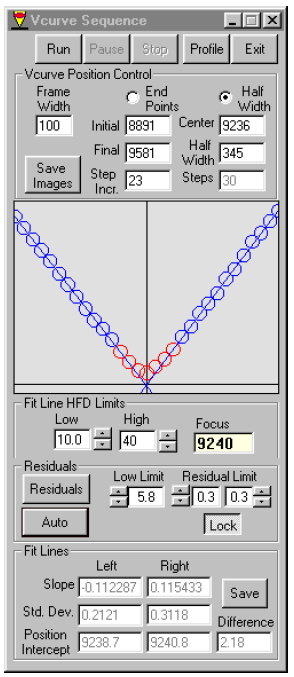
\includegraphics[width = 6.5cm]{V-curve}
	\end{center}
	\caption{FocusMAX에서 V curve를 얻어 초점을 결정하는 모습 \cite{weber2001fast}.}
	\label{fig:V-curve}
\end{figure}

\clearpage

\subsection{기존 제품 분석}

Fig. \ref{fig:microtouch}\가 바로 미국의 Starizona사에서 판매하는 Micro Touch  제품이다. Fig. \ref{fig:microtouch_3}\가 Micro Touch Autofocuser Hand Control system (Wired)이고, USB 케이블로 컴퓨터와 연결하여 ASCOMㅈ을징지원하는 소프트웨어에서 제어가 가능하다.  Fig. \ref{fig:microtouch_3}\는 Feather touch focuser에 모터를 장착한 모습이다. 

%%%%%%%새로 그림 추가함 (박기현샘)

\begin{figure}[H]
		\begin{subfigure}{0.45\textwidth}
		\begin{center}
			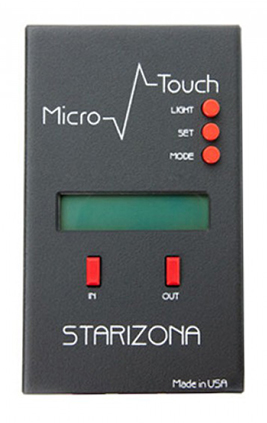
\includegraphics[width=0.6\linewidth]{microtouch_3} 
		\end{center}			
			\caption{Micro touch hand control system (Wired)}
			\label{fig:microtouch_3}
		\end{subfigure}
		\begin{subfigure}{0.45\textwidth}
		\begin{center}			
			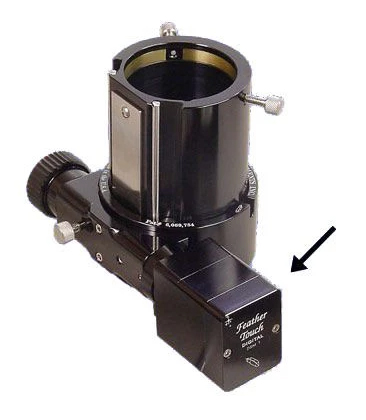
\includegraphics[width=0.75\linewidth]{microtouch_4}
		\end{center}
			\caption{Feather touch focuser with motor}
			\label{fig:microtouch_4}
		\end{subfigure}
		\caption{Starizona사에서 개발하여 판매하는 Micro touch 제품}
		\label{fig:microtouch}
\end{figure}


Fig. \ref{fig:microtouch_3}의 Micro touch 핸드 컨트롤러에 보이는 붉은 색 두 버튼(IN, OUT)은 각각 초점을 맞추기 위해 모터를 정방향, 역방향으로 회전시키는 버튼이다. Micro Touch는 버튼을 눌러 동작시킬 수 있을 뿐 아니라 USB(Universal serial port) 포트를 통해 PC와 연결하여 ASCOM driver 호환 소프트웨어를 통히 모터를 돌려 초점을 조절할 수 있다. 

%를 통해  수동 혹은 자동으로 작동시켜 IN 또는 OUT의 명령을 내렸을 경우, 모터 초점 조절 장치가 작동하게 된다. 이 모터 초점 조절 장치는 모터를 움직여 천체망원경의 경통의 길이를 조절할 수 있도록 한다. 경통의 길이가 변화하면 그에 따라서 빛이 퍼지는 정도가 달라지므로 이를 잘 조정하면 망원경으로 관측하는 천체의 초점을 맞출 수 있다.
하지만 이 제품은 다음과 같은 단점이 있다. 

첫째, Micro Touch 핸트 컨트롤러는 디스플레이를 이용하여 사용하는 사람들이 편하게 사용할 수 있도록 하였다. 2x16 LCD(Liquid-crystal display) displayer를 사용하여 문자 표현이 제한적이어서 여러 상황을 표현하는데 어려움이 있다. 

둘째, 제품의 크기가 매우 커서 한 손으로 잡고 조작하는데 불편하다. 핸드 컨트롤러라고 부르기에 적합하지 않을 정도로 너무 크게 설계되었다. 

셋째, Micro Touch 핸드 컨트롤러는 모터를 조절하는 것에도 한계가 있다. 자신의 회사에서 판매하는 모터를 회전시키는 데는 문제가 없으나 많은 전류를 필요로하는 모터는 탈조가 나서 사용할 수 없다. 또한 microstepping을 바꿀 수 없다. 

이렇게 가격도 비싸고 단점이 있는 Micro Touch 컨트롤러를 대체하기 위해 한 아마추어 천문가가 NanoFocus(https://atik.kr/nanofocus/)를 만들어 판매하고 있기도 한데 ASCOM으로 직접 제어할 수 있는 소프트웨어가 개발되어 있지 않은 것이 단점이다. 

본 연구는 기존의 제품들과 완벽하게 호환되며, 단점을 개선한 GS-touch를 제작하였으며, 그 응용 가능성은 매우 크다고 볼 수 있다. 


\subsection{제작을 위한 재료 선정}

기존에 출시되어 있는 모터 포커서 컨트롤러의 장점은 그대로 구현하고, 단점을 보완한 모터 포커서 컨트롤러를 제작하기 위하여 아두이노(Arduino)를 이용하였다. 아두이노는 오픈 소스를 기반으로 한 단일 보드 MCU(MicroController Unit) 보드와 관련 개발 도구 및 환경을 말한다. 2005년 이탈리아의 IDII(Interaction Design Institutelvera)에서 하드웨어에 익숙지 않은 학생들이 자신들의 디자인 작품을 손쉽게 제어할 수 있게 하려고 고안된 아두이노는 처음에 AVR을 기반으로 만들어졌으며, 아트멜 AVR 계열의 보드가 현재 가장 많이 판매되고 있다. ARM 계열의 Cortex-M0(Arduino M0 Pro)과 Cortex-M3(Arduino Due)를 이용한 제품도 존재한다. 현재 출시되어 있는 아두이노 보드 (Arduino board)들을 Table \ref{table:arduino_boards}에 나타내었다. 최근에는 이 보드들과 호환되는 저렴한 아두이노 호환 보드들도 판매되고 있으며, 드라이버만 제대로 설치되면 사용상 큰 문제는 없다. 

\begin{table}[ht]
	\caption{Arduino boards. \cite{wiki-arduino}}
	\begin{tabular}{c|l|l}
	\toprule[1pt]
		& MCU        & Arduino boards                            \\ 
		\toprule[1pt]
	
		\multirow{5}{*}{AVR} & ATmega168  & Pro(168), Mini(168), LilyPad (168V)                                     \\
		& ATmega328  & UNO, Fio, Nano, Pro(328), Mini(328, Rev5, 5V), Pro Mini, LilyPad (328V) \\
		& ATmega2560 & Mega 2560, Mega ADK                                                     \\
		& ATmega32U4 & Yún, Leonardo, Esplora, Micro                                           \\
		& ATtiny85   & GEMMA                                                                   \\ 
		\midrule[1pt]
		\multirow{2}{*}{ARM} & Cortex-M0+ & Zero, Zero PRO, M0, M0 PRO                                              \\
		& Cortex-M3  & Due      \\
	\bottomrule[1pt]   
	\end{tabular}
	\label{table:arduino_boards}
\end{table}

아두이노는 다수의 스위치나 센서로부터 값을 받아들여, LED나 모터와 같은 외부 전자 장치들을 통제함으로써 환경과 상호작용이 가능한 물건을 만들어 낼 수 있다. 임베디드 시스템 중의 하나로 쉽게 개발할 수 있는 환경을 이용하여, 장치를 제어할 수 있다. 아두이노 IDE (통합 개발 환경, Integrated Development Environment)을 제공하며, 소프트웨어 개발과 실행 코드 업로드도 제공한다 \cite{wiki-arduino}. 

포커서를 구동하기 위한 모터는 스테핑 모터 (spetting motor)를 사용하였다. 선풍기와 같이 우리가 실생활에서 볼 수 있는 모터는 대부분 DC 모터(direct current motor)이다. DC 모터는 전류가 흐르는 상태일 때 코일에 의해 계속 회전하는 원리를 사용하고 있기 때문에 원하는 위치나 각도에서 정지시키는 것이 어렵다. 때문에 망원경의 초점을 조절할 때에는 DC 모터를 사용하는 경우 정밀하게 회전을 제어하는데 어려움이 따른다. 

스테핑 모터의 여러 가지 특성은 정밀하게 제어해야 하는 포커서에 적합하다. 스테핑 모터는 그 상세한 종류에 따라 모양은 다르게 생겼지만 대부분의 스테핑 모터를 차지하는 PM형 모터의 경우 회전축에는 영구자석이 붙어있어 회전자(rotor)를 이루고, 바깥쪽에는 일정한 각도로 부착되어있는 전자석이 존재하여 고정자(Stator)를 이루게 된다. 외부에서 각 선에 전류를 흘려보내면, 전자석이 작동하여 회전자를 움직이게 만드는 원리로 움직인다. 쉽게 말하자면 전류 펄스로 제어되는 움직임이 DC 모터와 비교했을 때 스테핑 모터의 가장 큰 특징이다. 때문에 고정자들은 그 사이의 각도가 일정한 성질과 더해 한번 펄스를 쏠 때마다 일정한 각도를 움직이게 되며, 같은 양의 펄스를 주면 항상 같은 거리를 이동하므로 정확한 거리 계산에 용이하다.

또한 모터에 펄스형태가 아닌 선형으로 전류를 가하게 되면 안쪽의 회전자는 그대로 고정되어 힘을 받게 된다. 이 때 받는 힘의 크기를 홀적 토크라고 하며, 펄스 형태의 전류가 가해지지 않으면 모터는 움직이지 않고 정지한 상태를 유지한다. 이를 이용한 스테핑 모터의 또다른 특징이 바로 microstepping이다. 대부분의 스테핑 모터는 고정자의 전자석이 배치된 개수가 200개로 고정이 되어있어 한번 펄스를 가할 때 360/200인 1.8도(이를 single step, 혹은 full step이라 한다)를 움직이게 된다. 하지만 가하는 총 전류에 비해 약한 전류변화를 일으키면 full step에 비해 적은 각도 변화를 일으키게 되고, 이를 여러 단계로 나눈 것이 microstepping이다. 이를 활용하면 망원경의 특성에 따라 적절하게 모터의 힘과 속도, 위치의 정확성을 개선할 수 있다.

microstepping 뿐만 아니라 모터의 정확성과 힘에 관여하는 요소는 많이 존재한다. 대체적으로  모터에 가해지는 전류 펄스의 크기가 커지게 되기 때문에 전압에 비례해 토크가 커지게 된다. 또한, 모터의 속도는 가한 총 펄스에 비례하기 때문에 속도가 빨라지게 되면 가하는 펄스의 관성에 약해지게 되고 탈조현상이 일어날 가능성이 커지게 되며, 모터의 토크도 약해지게 된다. 비슷한 원리로, 전류 펄스의 크기를 약하게 만드는 microstepping 또한 모터의 토크를 저하시키게 된다.
